\subsection{Metody přímého vyhledávání}\label{direct-search}
Z metod přímého vyhledávání popíšeme \textit{generalised pattern search} (dále jen GPS) metodu \cite{Audet2002} a~krátce zmíníme také \textit{mesh adaptive direct search} (dále jen MADS) metodu \cite{Audet2006}.

Pro popis algoritmu GPS je nutné definovat síť, pomocí níž je pak popsáno prohledávání prostoru v~rámci GPS. Buďte $ \mathbf{G} \in \mathbb{R}^{n \times n} $ a $ \mathbf{Z} \in \mathbb{Z}^{n \times p} $. Nechť  každý vektor z $ \mathbb{R}^{n} $ lze vyjádřit jako lineární kombinaci sloupců matice $ \mathbf{Z} $ (vnímaných jako vektory) tak, že všechny koeficienty v této lineární kombinaci jsou nezáporné. Dále označme $ \mathbf{S} = \mathbf{G} \mathbf{Z}$. Síť $ \mathbf{M} $ generovanou pomocí $ \mathbf{S} $ středovanou v bodě $ \vec{x} $ definujeme jako
\begin{equation}
	\mathbf{M} = \left\{ \vec{x} + \delta \, \mathbf{S} y \, | \, y \in \mathbb{N}^p \right\},
\end{equation}
kde $ \delta $ je parametr, jenž budeme nazývat síťový krok \cite{BBO-textbook, Audet2002}. V jednotlivých iteracích algoritmu GPS se obecně mění tvar sítě, jelikož je vždy středována v bodě představující nejlepší odhad v dané iteraci, dále se také mění velikost síťového kroku. Označíme-li $ \vec{x}_k $, resp. $ \delta_k $ jako odhad řešení, resp. síťový krok  v $ k $-té iteraci, můžeme definovat síť v $ k $-té iteraci označenou $ \mathbf{M} _k$, tj.
\begin{equation}
	\mathbf{M} _k = \left\{ \vec{x}_k + \delta_k \, \mathbf{S} y \, | \, y \in \mathbb{N}^p \right\}.
\end{equation}
Poznamenejme, že sloupce výše definované matice $ \mathbf{S} $ lze chápat jako možné směry, kterými lze v rámci GPS prohledávat prostor hodnot optimalizačních parametrů \cite{BBO-textbook, Audet2002}.

Po inicializaci nutných počátečních parametrů je samotný algoritmus GPS v každé iteraci rozdělen do dvou hlavních kroků. Prvním krokem je tzv. hledání (anglicky \textit{search step}). Během kroku hledání je pomocí strategie blíže specifikované uživatelem vybrána konečná množina kandidátních síťových bodů, v nichž je vyčíslena účelová fukce. Pokud žádná z vypočtených hodnot nepředstavuje zlepšení oproti hodnotě $ f(\vec{x}_k) $, nastává krok průzkumu (anglicky \textit{poll step}). V kroku průzkumu je účelová funkce vyčíslena ve všech sousedních síťových bodech bodu $ \vec{x}_k $. V případě, že ani pak žádná z vypočtených hodnot nepředstavuje zlepšení oproti hodnotě $ f(\vec{x}_k) $, nastavíme $ \vec{x}_{k+1} = \vec{x}_k $ a snížíme hodnotu síťového kroku, tedy  $ \delta_{k+1} < \delta_k $. Pokud však v kroku hledání nebo v kroku průzkumu najdeme takový bod, pro který dojde k vylepšení odhadu řešení, označíme tento bod jako $ \vec{x}_{k+1} $ a zvýšíme hodnotu síťového kroku, tedy  $ \delta_{k+1} > \delta_k $ \cite{BBO-textbook, Audet2002}.

Výše popsané změny v každé iteraci vždy definují novou síť $ \mathbf{M} _k$, která se během algoritmu GPS obecně mění. Algoritmus je ukončen, když je splněno $ \delta_{k+1} < \varepsilon $ pro uživatelem specifikované $ \varepsilon > 0 $. Lze ukázat, že během GPS algoritmu konverguje krok sítě limitně k nule a za splnění vhodných předpokladů odhady řešení konvergují ke stacionárnímu bodu účelové funkce, detaily lze najít v \cite{BBO-textbook}. Podotkněme, že konvergence GPS je dokázána pro úlohy bez vazeb \cite{BBO-textbook}.

\begin{figure}[H]
	\centering
	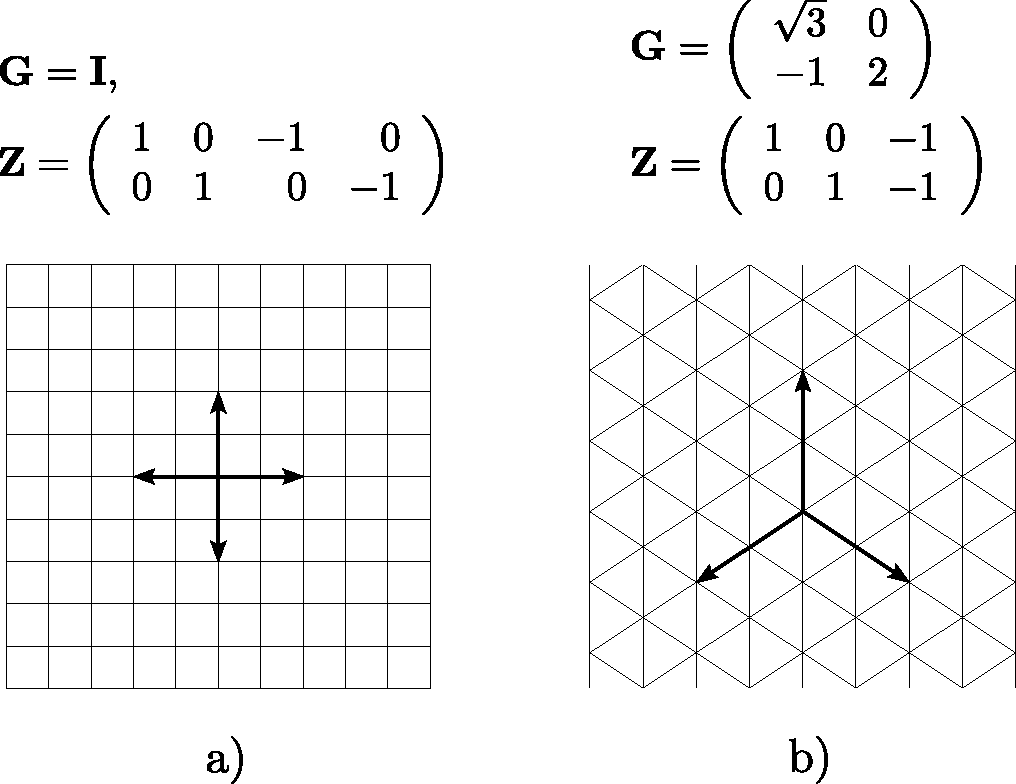
\includegraphics[width=0.7\textwidth]{figures/gps.pdf}
	\caption{Examples of search sets and meshes in R2 with
		$\delta^k$  obtained by the directions D = GZ; the mesh points
		are at the intersections of the lines and the arrows represent
		the poll set a) is that of the CS algorithm}
	\label{fig:gps}
\end{figure}


\begin{algorithm}[H]
	\caption{Generalized Pattern Search (GPS)}\label{GPS}
	\begin{algorithmic}[1]
		\Require Function $f: \mathbb{R}^n \to \mathbb{R}$, initial point $x^0$, initial mesh size parameter $\delta^0$, positive spanning matrix $D$, mesh size adjustment parameter $\tau \in (0, 1)$, stopping tolerance $\epsilon_{\text{stop}}$, iteration counter $k \gets 0$
		\Ensure Approximate solution $x^*$
		
		\Procedure{GPS}{$x^0$}
		
		\While{$\delta^k > \epsilon_{\text{stop}}$}
		
		\Algphase{1. Search}
		\State Define a finite subset $S^k$ of the mesh $M^k$
		\If{$f(t) < f(x^k)$ for some $t \in S^k$}
		\State Set $x^{k+1} \gets t$ and $\delta^{k+1} \gets \tau^{-1} \delta^k$
		\State \textbf{continue}
		\Else
		\State Go to Poll step
		\EndIf
		
		\Algphase{2. Poll}
		\State Select a positive spanning set $D^k \subseteq D$
		\State Define $P^k = \{x^k + \delta^k d : d \in D^k\}$
		\If{$f(t) < f(x^k)$ for some $t \in P^k$}
		\State Set $x^{k+1} \gets t$ and $\delta^{k+1} \gets \tau^{-1} \delta^k$
		\Else
		\State $x^k$ is a mesh local optimizer
		\State Set $x^{k+1} \gets x^k$ and $\delta^{k+1} \gets \tau \delta^k$
		\EndIf
		
		\Algphase{3. Termination}
		\If{$\delta^{k+1} \leq \epsilon_{\text{stop}}$}
		\State \textbf{terminate}
		\Else
		\State Increment $k \gets k+1$ and continue
		\EndIf
		
		\EndWhile
		\EndProcedure
	\end{algorithmic}
\end{algorithm}


Dále krátce zmíníme metodu MADS, která představuje vylepšení metody GPS. Narozdíl od metody GPS, algoritmus MADS umožní během kroku průzkumu obecně zkoumat hodnoty účelové funkce ve směrech, které tvoří hustou podmnožinu v $ \mathbb{R}^{n} $ \cite{BBO-textbook, derivative-free-review}. Toto zobecnění vylepšuje konvergenci algoritmu a umožňuje dokázat konvergenci MADS i pro úlohy s vazbami, kdy je účelová funkce modifikována na extrémní bariérovou funkci \ref{eq:extreme barrier}. Detaily týkající se algoritmu a fungování metody MADS lze najít např.~v~\cite{BBO-textbook}.



\begin{figure}[H]
	\centering
	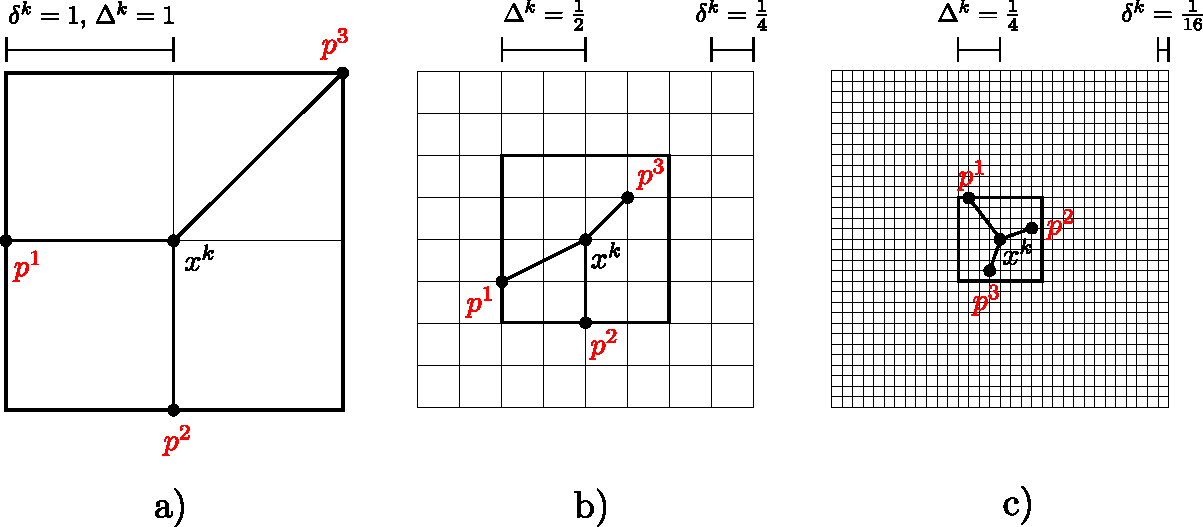
\includegraphics[width=0.99\textwidth]{figures/mads.pdf}
	\caption{Examples of search sets and meshes in R2 with
		$\delta^k$  obtained by the directions D = GZ; the mesh points
		are at the intersections of the lines and the arrows represent
		the poll set a) is that of the CS algorithm}
	\label{fig:mads}
\end{figure}



\begin{algorithm}[H]
	\caption{Mesh Adaptive Direct Search (MADS)}\label{MADS}
	\begin{algorithmic}[1]
		\Require Function $f_{\Omega}: \mathbb{R}^n \to \mathbb{R} \cup \{\infty\}$, initial point $x^0 \in \Omega$, initial frame size parameter $\Delta^0$, positive spanning matrix $D$, mesh size adjustment parameter $\tau \in (0,1)$, stopping tolerance $\epsilon_{\text{stop}}$, iteration counter $k \gets 0$
		\Ensure Approximate solution $x^*$
		
		\Procedure{MADS}{$x^0$}
		
		\While{$\Delta^k > \epsilon_{\text{stop}}$}
		
		\Algphase{1. Parameter Update}
		\State Set the mesh size parameter $\delta^k = \min \{\Delta^k, (\Delta^k)^2\}$
		
		\Algphase{2. Search}
		\State Define a finite set $S^k \subset M^k$ such that:
		\If{$f_{\Omega}(t) < f_{\Omega}(x^k)$ for some $t \in S^k$}
		\State Set $x^{k+1} \gets t$ and $\Delta^{k+1} \gets \tau^{-1}\Delta^k$
		\State \textbf{continue}
		\Else
		\State Go to Poll step
		\EndIf
		
		\Algphase{3. Poll}
		\State Select a positive spanning set $D_{\Delta^k}$ and define:
		\State $P^k = \{x^k + \delta^k d : d \in D_{\Delta^k}\}$, a subset of the frame $F^k$ with extent $\Delta^k$
		\If{$f_{\Omega}(t) < f_{\Omega}(x^k)$ for some $t \in P^k$}
		\State Set $x^{k+1} \gets t$ and $\Delta^{k+1} \gets \tau^{-1}\Delta^k$
		\Else
		\State Set $x^{k+1} \gets x^k$ and $\Delta^{k+1} \gets \tau\Delta^k$
		\EndIf
		
		\Algphase{4. Termination}
		\If{$\Delta^{k+1} \leq \epsilon_{\text{stop}}$}
		\State \textbf{terminate}
		\Else
		\State Increment $k \gets k+1$ and continue
		\EndIf
		
		\EndWhile
		\EndProcedure
	\end{algorithmic}
\end{algorithm}